En este capítulo se detalla el proceso de desarrollo del proyecto. En primer lugar, se analizarán los requisitos del proyecto para definir la arquitectura general del sistema. Luego se describirán el análisis, el diseño y la complementación de los componentes. Por último, se mostrarán datos ofrecidos por las herramientas de soporte al desarrollo.
 
 
 desarrollo.
  
\section{Análisis de Requisitos}


En esta aplicación móvil para actividades a campo abierto objetivo de este proyecto, se establecieron una seria de requisitos generales que debería cumplir la aplicación.\\

El registro del usuario para poder comenzar a usarla.\\

La creación de puntos de interés marcados en un mapa con nombre, descripción y un punto en el mapa con o sin señal GPS clasificados en tipo, caza o pesca. \\

Se podrán guardar las rutas seguidas por un usuario en sus caminatas por cualquier tipo de terrero.\\

El usuario también podrá crear grupos con los usuarios que quiera y los integrantes del mismo poder añadir a otros, el resultado de esta funcionalidad es la que permitirá posteriormente  crear rutas conjuntas. Para crear una ruta conjunta primero se elige el grupo del que se hará el seguimiento y se enviarán  las invitaciones para participar en él a cada integrante del grupo. Estas invitaciones en el caso de ser aceptadas llevaran al usuario a un mapa y periódicamente se irán realizando actualizaciones de las posiciones del resto de integrantes del grupo anteriormente indicado. Finalmente se podrán ver las rutas conjuntas igual que las individuales.
\subsection{Actores}

Los únicos actores que se presentan en la  aplicación son los siguientes:
\begin{itemize}
\item \textbf{Usuario no  autenticado}.Usuario que no está autenticado en la aplicación y que
se le permite registrarse en el  sistema o iniciar sesión si la ya se registro en otro momento.
\item \textbf{Usuario  autenticado}.Usuario autenticado que puede acceder a todas as funcionalidades
del sistema.
\end{itemize}
\subsection{Casos de uso}
A continuación, en esta sección, se exponen los requisitos funcionales que surgen de los requisitos generales planteados en el punto anterior.
\subsubsection{• Usuario no autenticado}
\begin{itemize}
\item\textbf{ \textit{R1}  Registrarse en la aplicación.}
 El usuario podrá darse de alta en el sistema
introduciendo sus datos en el formulario que se le indican. Una vez registrado se iniciará sesión
automáticamente con el nuevo perfil.

\item \textbf{\textit{R2} Iniciar sesión en la aplicación. }
El usuario ya registrado podrá, con
sus credenciales, autenticarse en el  sistema. Se pedirá o nombre del usuario la aplicación y  su contraseña. Se guardará el estado en el terminal hasta que el usuario decida desconectarse.
\end{itemize} 
\begin{figure}[H]
		\centering
		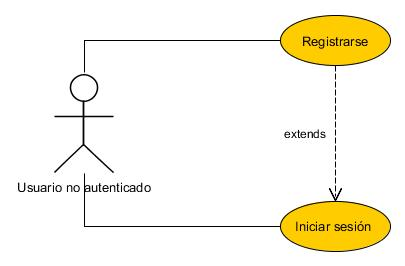
\includegraphics[width=0.75\textwidth] {usuario-no-autenticado.jpg}
		\caption{Casos de uso del actor Usuario No Autenticado }
	\end{figure}
\subsubsection{• Usuario  autenticado}
Para hacer un poco más comprensible dividiré los casos de uso del usuario autenticado por grupos funcionales.
\begin{itemize}
\item \textbf{Gestión de puntos de interés}\\
Aquí se describirán  los casos de uso relacionados con la gestión  de la  información del  los puntos de interés
\begin{itemize}
\item\textbf{\textit{ R-PDI-1 Guardar Punto De Interés caza}}, el usuario podrá guardar un punto concreto, de caza, asociado a un par de coordenadas pudiendo añadirle un nombre y una descripción.
\item\textit{ \textbf{R-PDI-2 Guardar Punto De Interés pesca}}, el caso de uno es similar al de anterior pero este es para el tipo de pesca.
\item \textbf{\textit{R-PDI-3 Eliminar PDI}}, el usuario podrá seleccionar un punto o una lista de puntos para ser borrados.
\item \textbf{\textit{R-PDI-4 Buscar los PDI}}, permite ver todos los puntos de interés de cada tipo por separado pintados en un mapa y pudiendo ciclar en ellos para conocer su nombre y descripción.
\end{itemize} 

\begin{figure}[H]
		\centering
		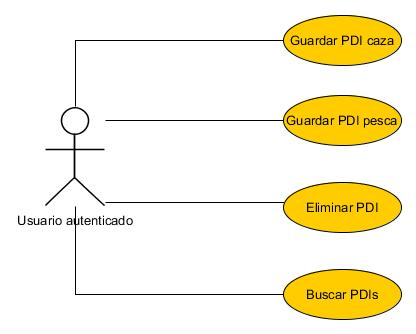
\includegraphics[width=0.75\textwidth] {PDI.jpg}
		\caption{Casos de uso de gestión de puntos de interés }
	\end{figure}
\item \textbf{Gestión de grupos}
\begin{itemize}
\item\textbf{ \textit{R-G-1 Crear grupo}}, el usuario crea un grupo con nombre único.
\item\textbf{\textit{ R-G-2 Añadir integrantes}}, el usuario busca en la base de datos los usuarios que quiere integrar en el grupo previamente creado.
\item \textbf{\textit{R-G-3 Eliminar integrantes}}, el usuario puede eliminar los integrantes que vea pertinentes.
\item \textbf{\textit{R-G-4 Ver grupos}}, el sistema listarla los grupos en los que el usuario está registrado.
\item \textbf{\textit{R-G-5 Ver integrantes grupo}}, el sistema permitirá ver los integrantes del grupo que el usuario indique , previo listado del caso de uso R-G-4. 

\end{itemize} 

\begin{figure}[H]
		\centering
		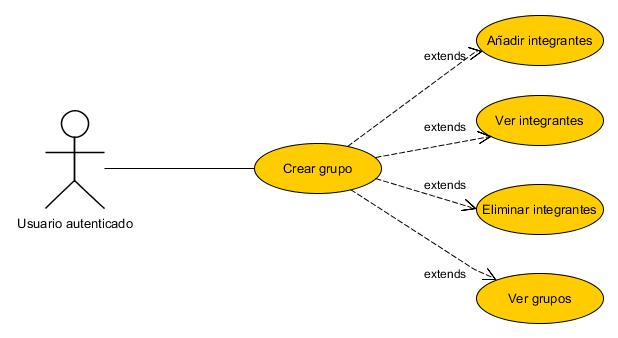
\includegraphics[width=0.75\textwidth] {grupo.jpg}
		\caption{Casos de uso de gestión de grupos de usuarios }
	\end{figure}
\item \textbf{Gestión de rutas,}el usuario iniciará una navegación privada siendo guardada la ruta seguida.
\begin{itemize}
\item \textbf\textit{{R-R-1 Crear ruta privada}}, el usuario registra la ruta con un nombre.
\begin{itemize}
\item \textbf{\textit{R-R-1.1}} Iniciar ruta, el sistema comienza a guardar las coordenadas por la que el usuario esta navegando y dibujando la ruta en el mapa. Las coordenadas se irán guardando periódicamente.
\item\textbf{ \textit{R-R-1.2}} Parar ruta, permite parar la navegación, tanto de guardar las coordenadas como de pintar la ruta seguida.
\item \textbf{\textit{R-R-1.3}} Guardar ruta, el sistema guarda los últimos puntos que quedaban sin actualizar y ejecuta el caso de uso ver ruta en el mapa(R-R-4).
\end{itemize}

\item \textbf{\textit{R-R-2 Crear ruta compartida}}, este caso de uso permite guardar la ruta seguida por el usuario y al mismo tiempo ver la posición del resto de integrantes de un grupo, anteriormente seleccionado, en tiempo real. Este caso de uso también enviaría a los integrantes del grupo una invitación a dicha ruta.
\begin{itemize}
\item \textbf{\textit{R-R-2.1 Iniciar ruta}}, se comienza a guardar y dibujar la ruta en el mapa. Por otra parte se comienza el seguimiento del resto de usuario que estén también navegando. Como también una actualización parcial de la ruta seguida en el servidor.
\item \textbf{\textit{R-R-2.2 Parar ruta}}, se para la navegación y se deja de actualizar la posición al resto de usuario de la ruta compartida.
\item \textbf{\textit{R-R-2.3 Finalizar ruta}}, se guardan los puntos que faltan de enviar al servidor y se deja de enviar datos al resto de integrantes.
\end{itemize}
\item \textbf{\textit{R-R-3 Listar rutas} }, permite al usuario ver todas las rutas realizadas tanto de manera privada como de manera compartida.
\item \textbf{\textit{R-R-4 Ver ruta en mapa}}, el sistema dibuja en un mapa la ruta seguida y previamente seleccionada.
\item \textbf{\textit{R-R-5 Eliminar ruta}}, permite al usuario borrar de la aplicación la ruta indicada.

\end{itemize} 
\end{itemize}
\begin{figure}[H]
		\centering
		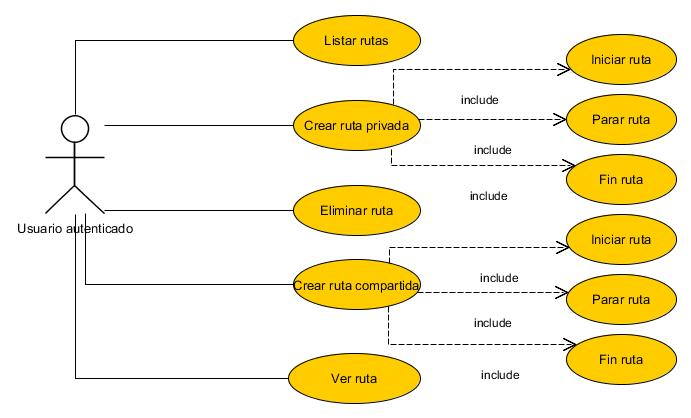
\includegraphics[width=0.75\textwidth] {rutas.jpg}
		\caption{Casos de uso de gestión de rutas }
	\end{figure}

\newpage
\section{Maquetas}
Comenzamos creando las maquetas de como debería que ser a interface del usuario.
Se busca que sea una interface simple y intuitiva.
Para esto, se intentarán seguir las pautas y usar lo  máximo posible los elementos de Material
Design [6].
Material Design es un lenguaje de diseñoo para distintas plataformas y dispositivos,
creada por el diseñador graco de Google Matas Duarte. Ofrece una guía  para ofrecer
a los usuarios una experiencia común y habitual entre distintas aplicaciones.


	
	
	
	\begin{figure}[htbp]
\begin{minipage}[b]{0.5\linewidth} %Una minipágina que cubre la mitad de la página
\centering
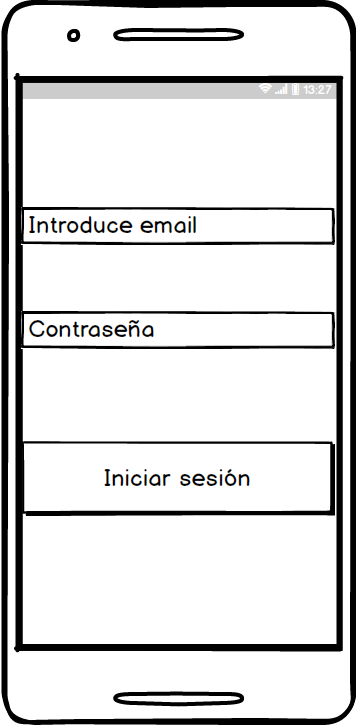
\includegraphics[width=6cm]{maqueta/Iniciar.png}
 \label{figura1}
\caption{Inisiar sesión}

\end{minipage}
\hspace{0.5cm} % Si queremos tener un poco de espacio entre las dos figuras
\begin{minipage}[b]{0.5\linewidth}
\centering
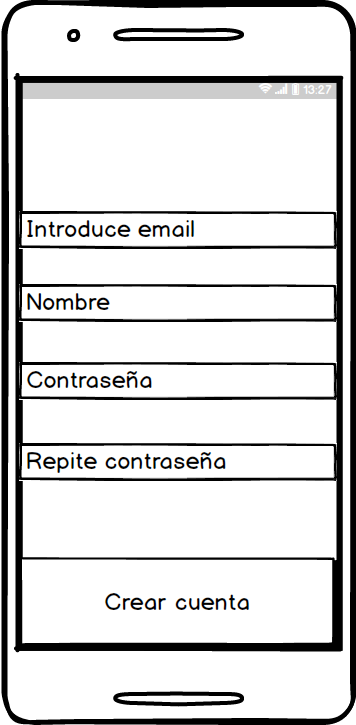
\includegraphics[width=6cm]{maqueta/Registrarse.png}
 \label{figura2}
\caption{Registrar usuario}

\end{minipage}
\end{figure}










	
	\begin{figure}[htbp]
\begin{minipage}[b]{0.5\linewidth} %Una minipágina que cubre la mitad de la página
\centering
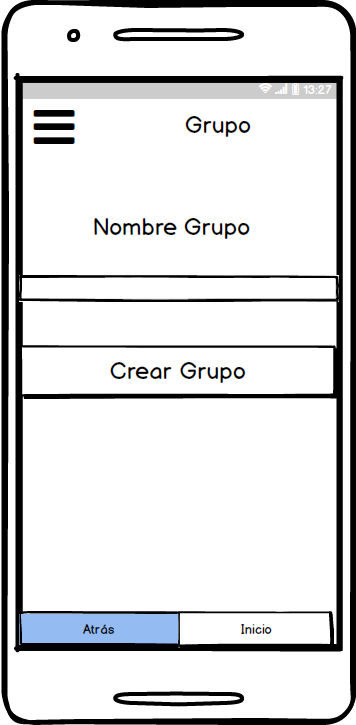
\includegraphics[width=6cm]{maqueta/Crear-Grupo.png}
 \label{figura1}
\caption{Crear grupo}

\end{minipage}
\hspace{0.5cm} % Si queremos tener un poco de espacio entre las dos figuras
\begin{minipage}[b]{0.5\linewidth}
\centering
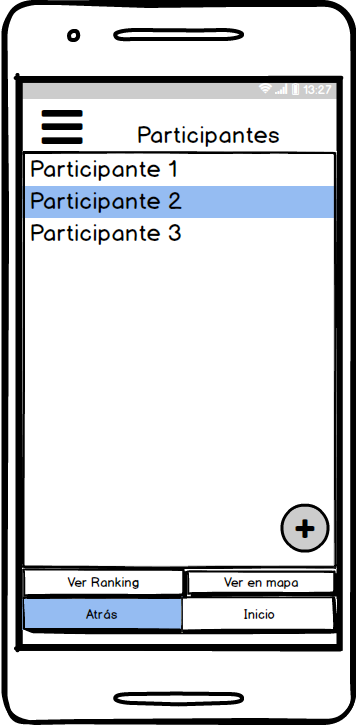
\includegraphics[width=6cm]{maqueta/Ver-Miembros-grupo.png}
 \label{figura2}
\caption{Añadir usuarios a grupo}

\end{minipage}
\end{figure}
	
	
	
	
	
	
	
	
	
	
	
	
	
	
	
	
	
	\begin{figure}[htbp]
\begin{minipage}[b]{0.5\linewidth} %Una minipágina que cubre la mitad de la página
\centering
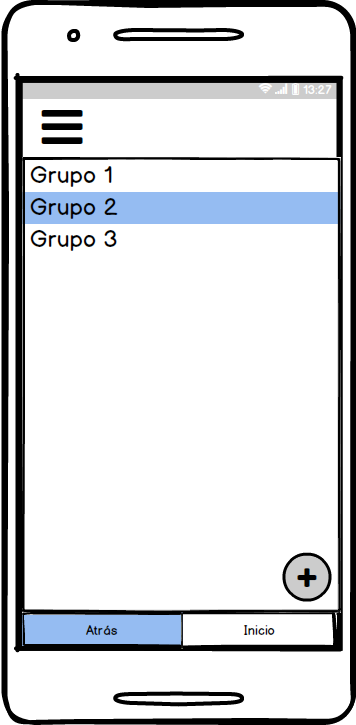
\includegraphics[width=6cm]{maqueta/lista-grupos.png}
 \label{figura1}
\caption{Listar grupos}

\end{minipage}
\hspace{0.5cm} % Si queremos tener un poco de espacio entre las dos figuras
\begin{minipage}[b]{0.5\linewidth}
\centering
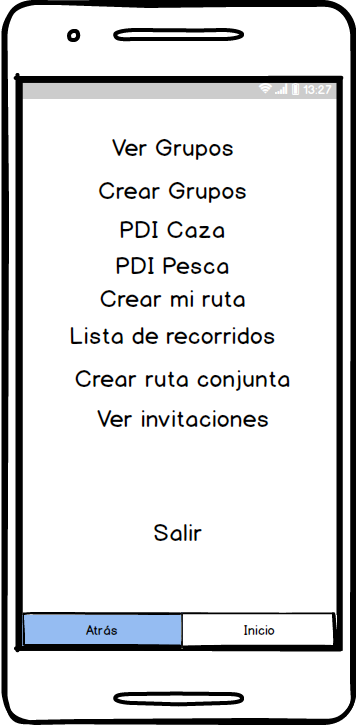
\includegraphics[width=6cm]{maqueta/opciones.png}
 \label{figura2}
\caption{Opciones generales}

\end{minipage}
\end{figure}
	















	\begin{figure}[htbp]
\begin{minipage}[b]{0.5\linewidth} %Una minipágina que cubre la mitad de la página
\centering
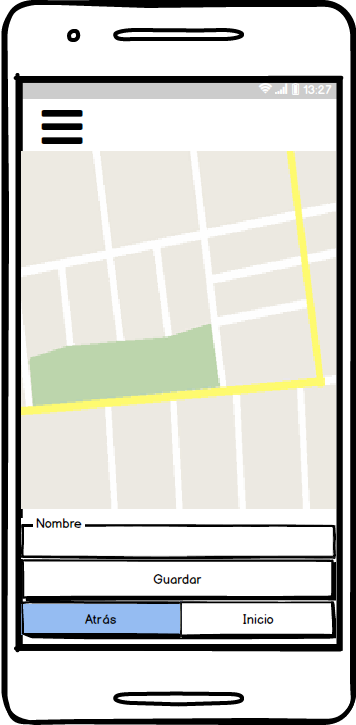
\includegraphics[width=6cm]{maqueta/pdi1.png}
 \label{figura1}
\caption{Crear PDI}

\end{minipage}
\hspace{0.5cm} % Si queremos tener un poco de espacio entre las dos figuras
\begin{minipage}[b]{0.5\linewidth}
\centering
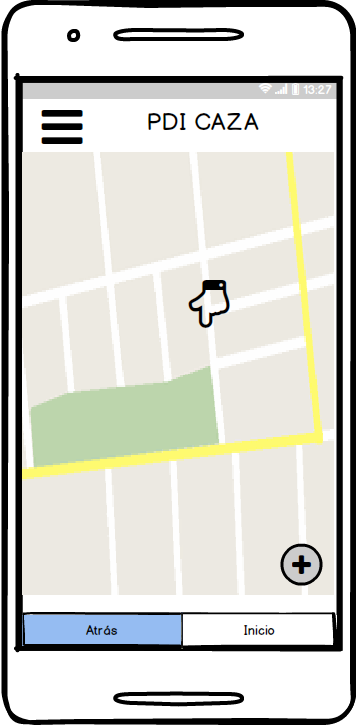
\includegraphics[width=6cm]{maqueta/pdi2.png}
 \label{figura2}
\caption{Visualizar PDIs}

\end{minipage}
\end{figure}
	

	\begin{figure}[htbp]
\begin{minipage}[b]{0.5\linewidth} %Una minipágina que cubre la mitad de la página
\centering
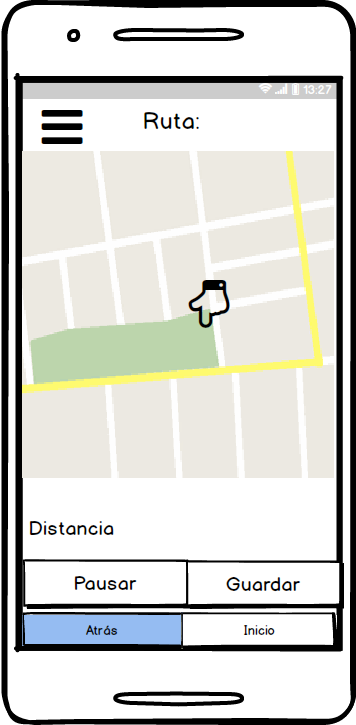
\includegraphics[width=6cm]{maqueta/Trayecto-actual.png}
 \label{figura1}
\caption{Ruta individual}

\end{minipage}
\hspace{0.5cm} % Si queremos tener un poco de espacio entre las dos figuras
\begin{minipage}[b]{0.5\linewidth}
\centering
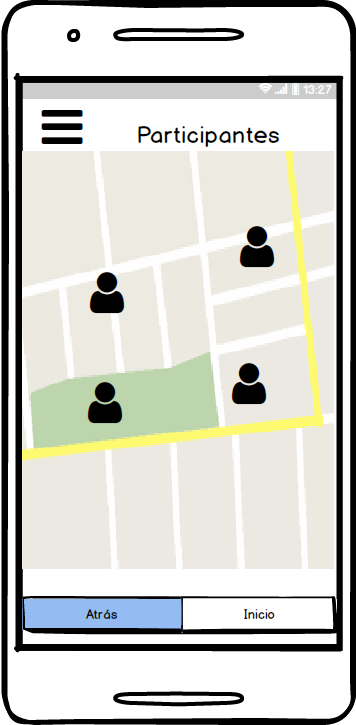
\includegraphics[width=6cm]{maqueta/Trayecto-actual-compartido.png}
 \label{figura2}
\caption{Ruta compartida}

\end{minipage}
\end{figure}



\newpage
\chapter{Diseño}
\section{Arquitectura propuesta}
\label{s:dev:arch}
 

En este capítulo se comentará el diseño de la aplicación de manera superficial, la arquitectura general, el
modelo de datos y también aspectos más concretos del diseño del servidor y da aplicación
móvil.

\

\subsection{Esquema general de la arquitectura}
La aplicación que estamos desarrollando seguirá la arquitectura
en tres capas. Este patrón arquitectónico cliente/servidor se diferencian tres
capas, una capa de interface de usuario , una capa de persistencia
y una capa intermedia llamada de servicios que permite la llamada de forma remota a la capa modelo(capa que contiene la lógica) por parte del cliente. Este esquema esta compuesto por:




\begin{figure}[H]
		\centering
		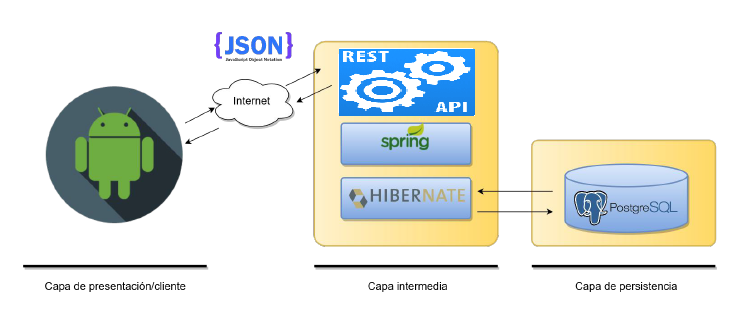
\includegraphics[width=0.75\textwidth] {arquitectura.png}
		\caption{Esquema general de la arquitectura del sistema }
	\end{figure}


\begin{itemize}
\item \textbf{Capa de presentación/cliente}:\\
Capa que  nos proporciona la información relacionada con los servicios que puede invocar el cliente. Es la encargada de comunicarse con las otras capas para guardar la información de cada usuario.En si es la capa con la que va a interactuar el usuario cada vez trabaje con esta aplicación.
\item \textbf{Capa intermedia:}\\
Esta capa es la encargada de enlazar la capa de persistencia con la capa de presentación/cliente. Lo que hace es recoger los datos que provienen de la base de datos, necesarios para satisfacer el servicio invocado y enviárselos al cliente.

\item \textbf{Capa de persistencia:}\\
Esta capa es la encargada de almacenar los datos del sistemas en la base de datos, además contiene todos los mecanismos de acceso a datos necesarios para poder hacer persistentes los datos.
 Esta capa debe ofrecer una interface que ayude a la comunicación con la capa intermedia, de manera que se abstraiga de la tecnología usada en el sistema de almacenamiento y no crea una dependencia con ella. Esta abstracción permitirá hacer cambios o actualizaciones en la tecnología sin afectar a otras capas con las que pudiera interaccionar en un futuro.\\
 


\end{itemize}
Un vez comentada la arquitectura general del sistema, pasaremos a comentar la capa intermedia un poco más a fondo ya que en ciertas ocasiones, la capa intermedia puede estar compuesta de N-capas(Arquitectura en N-capas). Ésta es una de esas ocasiones.

Los servidores que siguen el modelo Modelo-Vista-Controlador consiguen separar los datos de la  aplicación, la lógica de negocio  y el envío  de información por la red.
Ésta separación ayuda al desarrollo de la aplicación tanto a la hora de crear la como a la hora de hacer su mantenimiento ya que marca al desarrollador a colocar el código en una capa concreta. \\


Los componentes capas que componen al patrón MVC son:

\begin{itemize}
\item \textbf{Modelo:}\\
Está compuesta por clases que tienen acceso a los datos ofreciendo unos métodos que pueden ser usados de manera sencilla por las capas superiores. Éstos métodos son los encargados de acceder a la base de datos y proporcionar los datos persistentes.



\item \textbf{Vista:}\\

Esta formada por el interfaz donde se realizan las llamadas entre el servicio web, peticiones HTTP en las que la información va en formato JSON, y la aplicación cliente.

\item \textbf{Controlador:}\\
Esta capa será la encargada de implementar la lógica del interface llamando a las operaciones que ofrece el modelo y seleccionando la vista asociada a cada petición.



\end{itemize}


\section{Modelo de datos}

\section{Servidor}

Para que pudiera haber una comunicación entre la aplicación del cliente y la capa de persistencia hemos desarrollado una solución que se desplegará a través de un interface, al que se podrá acceder de manera remota y que permitirá tener acceso a las funcionalidades de la capa persistente.

La solución mencionada anteriormente será una aplicación, en java, que  usará Spring ya que facilita la creación de aplicaciones de forma cómoda y rápida.\\

Durante el desarrollo  de este proyecto el servidor ha sido desplegado en un proveedor de servidores virtuales llamado 
  DigitalOcean,ya que ofrece distintos lugares donde poder ubicar lo hemos decidido hacerlo en uno concreto de Alemania para que el ping fuera mas cercano y rápido.
\begin{figure}[H]
		\centering
		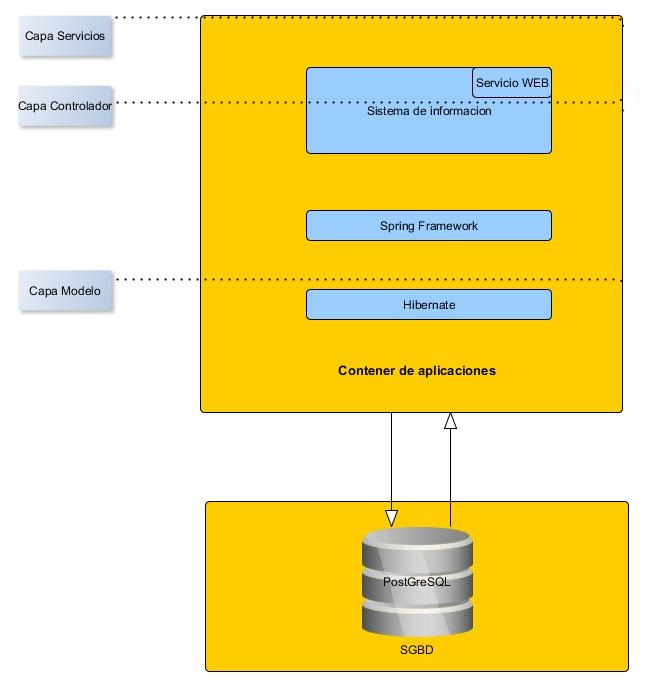
\includegraphics[width=0.75\textwidth] {arquitectura-servidor.jpg}
		\caption{Arquitectura del servidor }
	\end{figure}


\subsection{Servizo web}
A comunicacion farase a traves do paradigma Rest que e un estilo arquitectonico para
construr aplicacions distribudas inspirado nas caractersticas da web e que emprega
directamente HTTP para obtencion de datos. A traves das seguintes peticions HTTP
poderemos acceder os distintos recursos.


\begin{itemize}
\item Os metodos de acceso especican a accion que se quere realizar sobre un recurso. Desta
forma o usar GET solicitarase unha representacion do recurso pedido. PUT crea
unha nova representacion dun recurso e POST modifcaa. Tamen existe o metodo
DELETE que elimina o recurso especicado.
\item Dependendo do metodo que se empregue a ruta sobre a que se fai a peticion HTTP
e distinta. Tanto POST como DELETE realzanse sobre recursos especco, polo tanto
a ruta parecerase a : . PUT empregase sobre recursos
coleccion /recursos. O metodo GET pode ser usando tanto en recursos coleccion
como individuais.


\end{itemize}

\subsection{Organizacion dos paquetes}

\subsection{Transmision de Informacion}

\subsection{Xestion das clases persistentes}

\section{Aplicación Móvil}